\documentclass[a4paper]{report}
\usepackage{float}
\usepackage{geometry}
\usepackage{graphicx}
\usepackage{hyperref}
\usepackage{xepersian}
\newgeometry{left=1.4cm, right=1.4cm, bottom=2.0cm, top=2.0cm}
\settextfont[Scale=1.0]{XB Roya}

\title{زنجیره آسیب پارکینگ آنلاین و فرایند رزرو جایگاه \\ مهندسی نیازمندی‌ها،
خانم دکتر سپیده آدابی}
\author{علیرضا سلطانی نشان}

\begin{document}
\maketitle

\section{کاربرد}

هدف از انجام این تکلیف نمایش وابستگی اهداف به یکدیگر است. عوامل آن‌ها نیز در
رسیدن به اهداف دخیل هستند. پس اگر برای رسیدن به هدفی، عاملی بد عمل کند، می‌تواند
مانع رسیدن ما به هدف نهایی شود.

\section{هدف}

هدف در این سیستم بدست آوردن جایگاه پارکینگ برای کاربر است. کاربر می‌خواهد ساعت
۹:۳۰ فردا در جایگاه مناسب خودروی خود را در پارکینگ سازمان مورد نظر پارک کند.
برای این کار از روز قبل جایگاه مورد نظر خود را بایستی رزرو کند. رزرو می‌تواند در
دو حالت لحظه و هفتگی اتفاق افتد. کاربر بدون اپلیکیشن پارکینگ هوشمند نمی‌تواند
جایگاه پارک را به صورت آنلاین رزرو کند. همچنین شماره جایگاه پارک را کاربر انتخاب
نمی‌کند بلکه با استفاده از الگوریتم‌های مناسب، عادلانه‌ترین جایگاه پارک کاربر به
وی اختصاص می‌یابد.

کاربر بدون داشتن اپلیکیشن نمی‌تواند از خدمات پارکینگ آنلاین استفاده کند. کاربر
بدون ثبت پلاک جدید نمی‌تواند جایگاه پارکینگی را رزرو هفتگی یا لحظه‌ای کند. این
اهداف کاملاً به یکدگیر وابسته هستند.

\section{تعاریف}

\begin{itemize}
    \item \lr{G 1}: هدف نخست نصب موفق اپلیکیشن بر روی گوشی کاربر است.
    \item \lr{Agent 1}: وظیفه نصب بر عهده سیستم عامل اندروید می‌باشد.
    \item \lr{G 2}: احراز هویت موفقیت آمیز
    \item \lr{Agent 2}: تابع احراز هویت اپلیکیشن موبایل و ارسال درخواست به سیستم
    احراز هویت
    \item \lr{G 3}: ثبت یک پلاک جدید
    \item \lr{Agent 3}: تابع ثبت پلاک و دریافت اسناد خودرو از کاربر و ارسال آن
    به سرویس ثبت پلاک.
    \item \lr{G 4}: رزرو هفتگی/لحظه‌ای جایگاه پارک
    \item \lr{Agent 4}: انتخاب نوع رزرو و ارسال درخواست رزرو جایگاه به سرویس
    دریافت‌کننده درخواست کاربر.
    \item \lr{G 5}: دریافت شماره جایگاه پارک خودرو در پارکینگ سازمان به وسیله
    پیامک
    \item \lr{Agent 5}: بعد از دریافت درخواست رزرو جایگاه پارک، الگوریتم اختصاص
    جایگاه اجرا می‌شود و سپس شماره جایگاه پارکینگ برای کاربر پیامک می‌شود.
\end{itemize}

\begin{figure}[H]
  \centering
  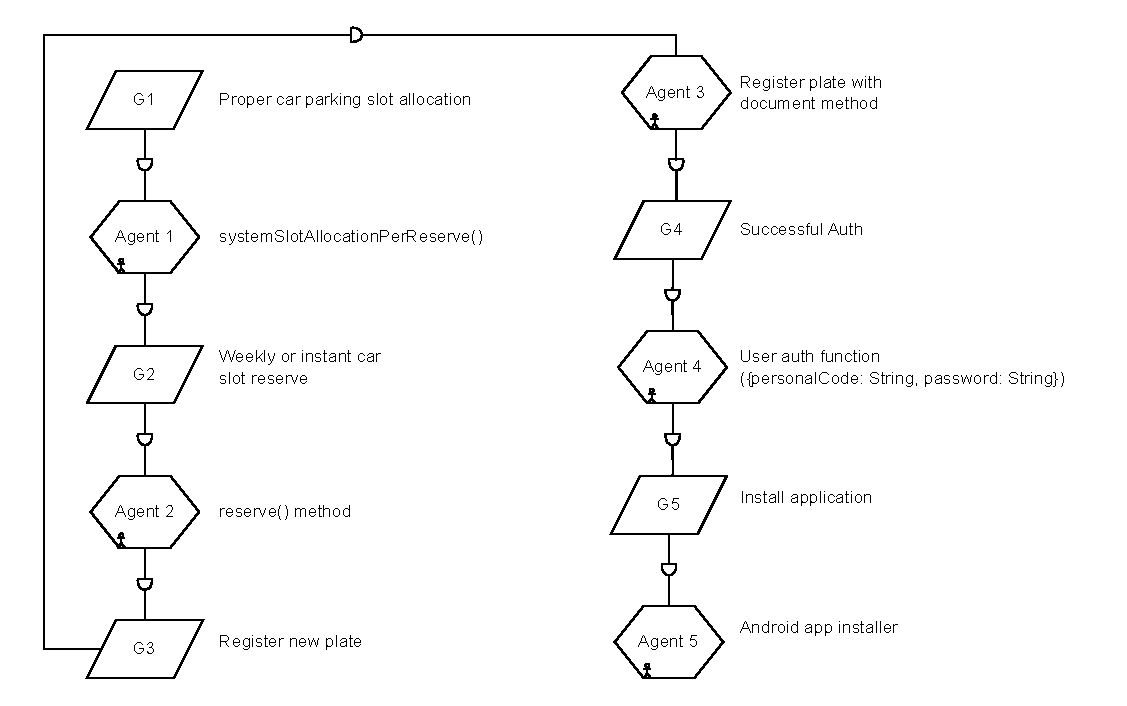
\includegraphics[width=0.75\textwidth]{threat_chain_smart_parking.drawio.pdf}
  \caption{نمودار زنجیره آسیب فرایند تخصیص جایگاه پارک}
\end{figure}

\end{document}